%% For Page Style :
\pagestyle{fancy}
\fancyhf{}
\fancyhead[LE]{\thepage}
\fancyhead[RO]{\thepage}
\fancyhead[RE]{\nouppercase{\textbf{\leftmark}}}
\fancyhead[LO]{\textbf{Tutorial BlankOnDev version 0.1005}}
\setlength{\parindent}{1cm}
\setlength{\parskip}{0.25cm}
%\fontsize{\normalsize}{baselineskip}

\chapter{Troubleshooting Migrasi Paket}
\label{chap:trouble_mig}

Pada bagian ini akan dijelaskan 2 permasalah terkait dengan aktifitas Migrasi paket dari Repositori Bazaar ke Repositori Github. Beberapa permasalahan yang akan dijelaskan pada upabab ini, akan diselesaikan dengan perintah \texttt{boidev bzr2git} atau \texttt{boidev bzr2git <cmd2>}.

\section{Paket github belum dikonverersi}
\label{sec:pkg-github-no-convert}
\noindent
Berikut contoh paket yang didorong ke github, tanpa dilakukan Konversi format :

\begin{figure}[H]
	\centering
	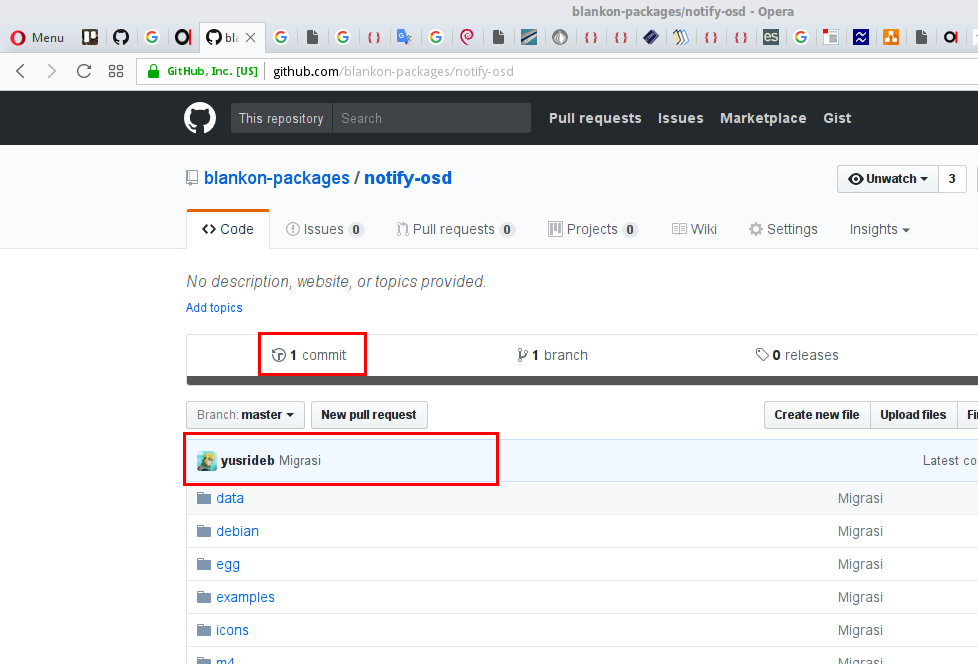
\includegraphics[width=12cm]{pkg-github-no-convert.png}
	\caption{Contoh paket yang diupload tanpa konversi format ke github}
	\label{fig:bab3_pkg-gihub-no-convert}
\end{figure}

\noindent
Untuk memperbaiki repositori ini, sebenarnya bisa langsung menghapus repositori di akun github, kemudian mengupload ulang paket yang sudah dikonversi ke format git. Jika hanya 1 paket mungkin tidak masalah, namun jika sudah terdapat repositori yang harus dihapus kemudian diupload ulang ke Github, maka beresiko salah hapus repositori. 

\noindent
Untuk melesaikan permasalahan seperti ini \textit{BlankOnDev Tools} menyediakan fitur untuk perbaikan repositori github yaitu dengan cara seperti yang ditunjukkan pada upabab \textit{\ref{sec:pre_impl_pros_mig}. Proses Migrasi Paket, bagian \ref{implm_4} dan bagian \ref{implm_5}}. berikut Ilustrasi penyelesaian masalah :

\subsection{Problem Solved dengan perintah \texttt{boidev bzr2git <cmd>}}
\label{sec:problem-solved1}
\noindent
Pada contoh ini nama paket yang bermasalah yaitu \textbf{notify-osd}, berikut daftar perintah yang digunakan untuk menyelesaikan masalah :
\begin{itemize}
	\item Perintah \texttt{boidev bzr2git branch \textbf{notify-osd}}
	\item Perintah \texttt{boidev bzr2git bzr-cgit \textbf{notify-osd}}
	\item Perintah \texttt{boidev bzr2git re-gitpush \textbf{notify-osd}}
	\item Perintah \texttt{boidev bzr2git git-check \textbf{notify-osd}}
\end{itemize}

\noindent
Rangkaian proses penggunaan perintah :

\begin{lstlisting}[language=ShellBash3]
$ boidev bzr2git branch notify-osd

Rilis Active : tambora

You want to Re-branch [y/n] : y

Bazaar re-branch for packages : "notify-osd"
Action re-branch for packages "notify-osd" 

======== Packages notify-osd has been finished to bzr branch ========

\end{lstlisting}

\begin{lstlisting}[language=ShellBash3]
$ boidev bzr2git bzr-cgit notify-osd

Rilis Active : tambora

Converting .... 


======== Packages notify-osd has been finished to convert ========

\end{lstlisting}

\begin{lstlisting}[language=ShellBash3]
$ boidev bzr2git re-gitpush notify-osd

Rilis Active : tambora

Re-push to GitHub .... 
----------------------------------------

re-push to git for packages "notify-osd" has success. 
\end{lstlisting}

\begin{lstlisting}[language=ShellBash3]
$ boidev bzr2git git-check notify-osd

Rilis Active : tambora
Check Repo [notify-osd] on github : repo_github = master, tambora 

git check repository for packages "notify-osd" | repo_github = master, tambora. 
\end{lstlisting}

\noindent
Hasil dari keempat perintah diatas yaitu :

\begin{figure}[H]
	\centering
	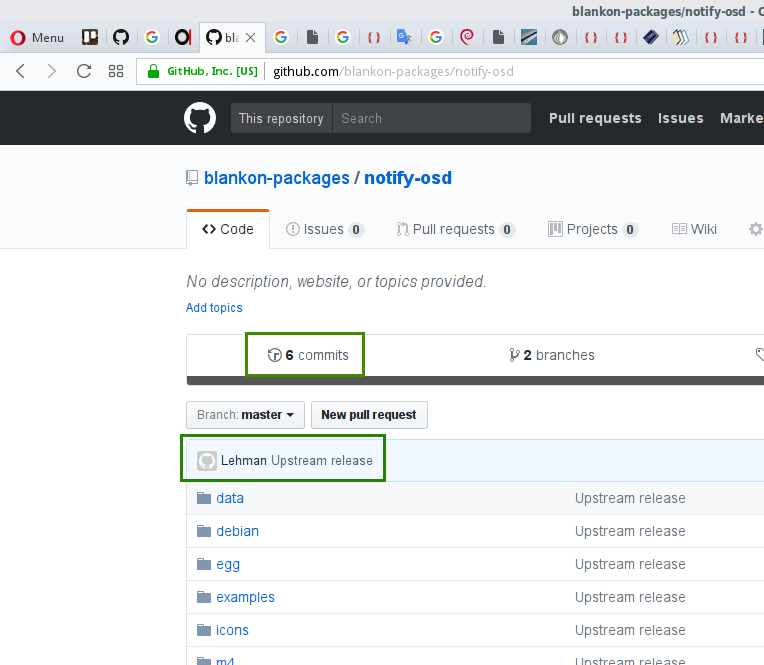
\includegraphics[width=95mm]{solved-github-no-convert.png}
	\caption{Penyelesaian masalah : Format paket belum dikonversi ke format git}
	\label{fig:bab3_solved1-gihub-no-convert}
\end{figure}

\pagebreak
\subsection{Problem Solved dengan perintah \texttt{boidev bzr2git}}}
\noindent
Pada bagian ini akan diilustrasi penyelesaian masalah mengunakan perintah \texttt{boidev bzr2git}. Berikut Ilustrasinya :


\begin{lstlisting}[language=ShellBash3]
yusrideb@pemaket:~$ boidev bzr2git

Rilis Active : tambora

---------------------------------------------------------------------------
Choose Action : 
---------------------------------------------------------------------------
1. All Packages
2. Specific Group Packages
3. Single Packages
Answer: 3

Enter packages name : notify-osd

Action re-branch for packages "notify-osd" 
[success] Action "bzr branch -> notify-osd" : 1
[success] Action "bzr convert git -> notify-osd" 1
[success] re-Action "bzr convert git -> notify-osd" 1
[success] Action "re-git push -> notify-osd" 
[success] Action "git check -> notify-osd" repo_github = master, tambora

========= Migration packages "notify-osd" has been finished =========
\end{lstlisting}

\noindent
Output Perintah :

\begin{figure}[H]
	\centering
	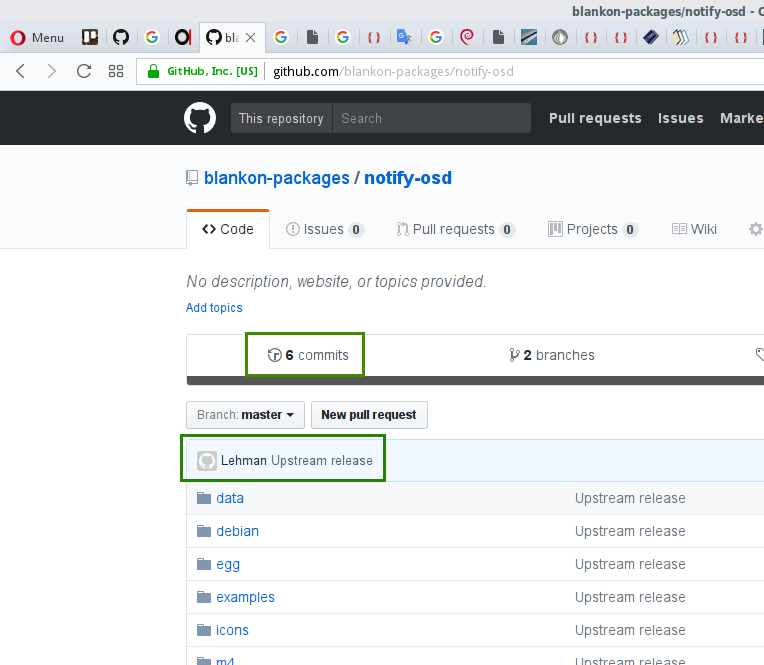
\includegraphics[width=95mm]{solved-github-no-convert.png}
	\caption{Penyelesaian masalah : Format paket belum dikonversi ke format git}
	\label{fig:bab3_solved2-gihub-no-convert}
\end{figure}

\section{Paket github hanya memiliki 1 jenis \textit{Branch}}
\label{sec:problem-solved2}
\noindent
Berikut contoh paket yang di dorong ke github, namun tidak dibuatkan branch ke rilis \textbf{tambora}, hanya branch \textbf{master} saja.

\begin{figure}[H]
	\centering
	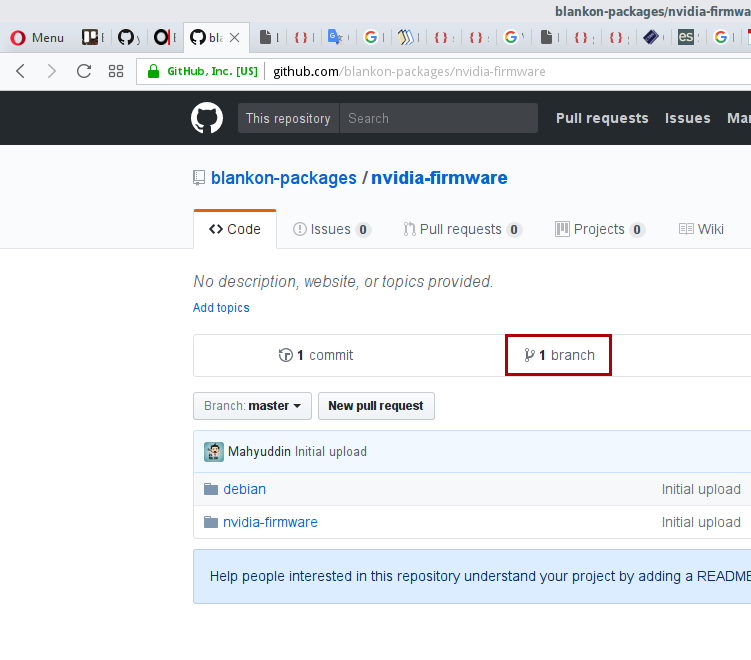
\includegraphics[width=8cm]{pkg-github-1-branch.png}
	\caption{Contoh paket yang diupload ke github, namun hanya memilik branch \textit{master}}
	\label{fig:bab3_github-1-branch}
\end{figure}

\noindent
Untuk memperbaiki repositori github seperti permasalah ini, dapat diselesaikan dengan seperti yang diilustrasi pada upabab \textit{\ref{sec:pkg-github-no-convert}}. Metode yang digunakan yaitu \hyperref[implm_4]{\textbf{Metode Split}} atau \hyperref[implm_5]{\textbf{Metode One-time}}. Pada bagian ini menggunakan \hyperref[implm_5]{\textbf{Metode One-time}}. Berikut ilustrasinya :

\begin{lstlisting}[language=ShellBash3]
$ boidev bzr2git

Rilis Active : tambora

---------------------------------------------------------------------------
Choose Action : 
---------------------------------------------------------------------------
1. All Packages
2. Specific Group Packages
3. Single Packages
Answer: 3

Enter packages name : nvidia-firmware

Action re-branch for packages "nvidia-firmware" 
[success] Action "bzr branch -> nvidia-firmware" : 1
[success] Action "bzr convert git -> nvidia-firmware" 1
Username for 'https://github.com': yusrideb
Password for 'https://yusrideb@github.com': 
[success] Action "git push -> nvidia-firmware" 1
[success] Action "git check -> nvidia-firmware" repo_github = master, tambora

=========== Migration packages "nvidia-firmware" has been finished ===========

\end{lstlisting}

\noindent
Hasil dari ilustrasi diatas :

\begin{figure}[H]
	\centering
	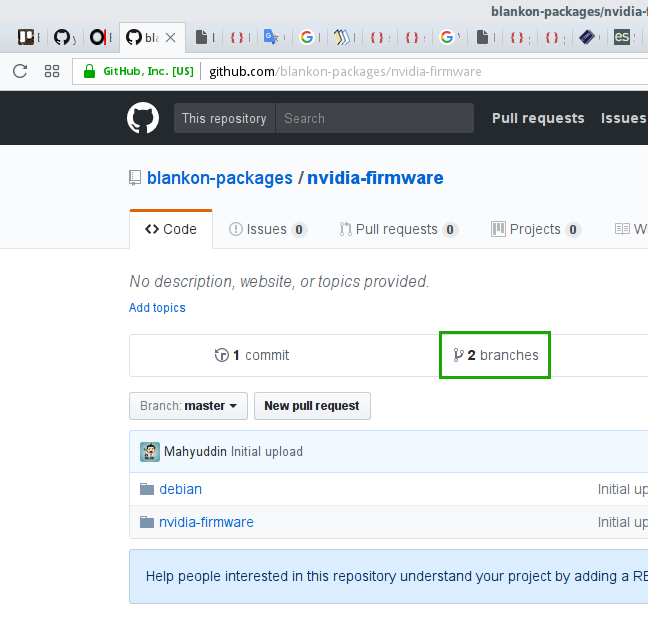
\includegraphics[width=10cm]{solved-github-1-branch.png}
	\caption{Penyelesaian Masalah : Repositori Github hanya memiliki type branch \textit{master}}
	\label{fig:bab3_solved-github-1-branch}
\end{figure}